\documentclass[final,5p,times,twocolumn,authoryear,11pt,nopreprintline]{elsarticle}
\usepackage[utf8]{inputenc}
\usepackage[T1]{fontenc}
\usepackage[spanish]{babel}
\usepackage{graphicx}
\usepackage{adjustbox}
\usepackage{amsmath,amssymb}
\usepackage{array,booktabs,tabularx}
\usepackage{mathtools}
\usepackage{microtype}
\usepackage{dblfloatfix}
\usepackage[hidelinks]{hyperref}
\usepackage{enumitem}
\urlstyle{same}
\setlength{\parindent}{1.27cm}
% Nombre del archivo .png y recuadro de reserva si no se ha exportado.
\newcommand{\figpng}[1]{\IfFileExists{imagenes/#1}{\includegraphics[width=\columnwidth]{imagenes/#1}}{\fbox{\parbox[c][4.0cm][c]{.90\columnwidth}{\centering Figura pendiente:\\ \texttt{\detokenize{#1}}}}}}
\newcommand{\fitcol}[1]{\resizebox{\columnwidth}{!}{#1}}
% APA: número de tabla destacado, título en cursiva.
\usepackage{caption}
\captionsetup[table]{name=Tabla,labelfont=bf,textfont=it,labelformat=simple,labelsep=newline,justification=raggedright,singlelinecheck=false}
\captionsetup[figure]{name=Figura,justification=raggedright,singlelinecheck=false}
\newcommand{\tituloProyecto}{Simulación numérica de un modelo SIRS rápido--lento acoplado a difusión de información y desinformación}
\begin{document}
\begin{titlepage}
\onecolumn
\centering
\vspace*{2cm}
{\large Universidad de Ingeniería y Tecnología}\\[0.2cm]
{\large Departamento Académico de Ciencias}\\[1.5cm]
{\Large \bfseries \tituloProyecto}\\[2cm]
\begin{minipage}{0.96\textwidth}
\centering
\large
\textbf{Curso:} Métodos Numéricos (CC2104)\\[0.3cm]
\textbf{Profesora:} Reynoso Quispe, Patricia\\[1cm]
\textbf{Integrantes:}\\[0.3cm]
{\small\begin{tabular}{@{}ll@{}}
Timana Carmona, Jose Manuel & 202510502 \quad (jose.timana@utec.edu.pe) \\[0.15cm]
Belevan Del Carpio, Santiago & 202310547 \quad (santiago.belevan@utec.edu.pe) \\[0.15cm]
Torres Baldoceda, Matias John & 202510029 \quad (matias.torres@utec.edu.pe) \\[0.15cm]
Davila Bazan, Santiago Sebastian & 202510442 \quad (santiago.davila@utec.edu.pe) \\[0.15cm]
Feijoo Gonzales, Carlos Augusto & 201910028 \quad (carlos.feijoo@utec.edu.pe)
\end{tabular}}
\end{minipage}
\vfill
\textbf{Fecha de entrega:} 18/10/2026
\vspace*{1cm}
\end{titlepage}
\twocolumn
\begin{frontmatter}
\title{\tituloProyecto}
\author[utec]{Timana Carmona, Jose Manuel}
\author[utec]{Belevan Del Carpio, Santiago}
\author[utec]{Torres Baldoceda, Matias John}
\author[utec]{Davila Bazan, Santiago Sebastian}
\author[utec]{Feijoo Gonzales, Carlos Augusto}
\address[utec]{Universidad de Ingeniería y Tecnología, Departamento Académico de Ciencias}
\end{frontmatter}
\section{Introducción}

En la actualidad, la propagación de enfermedades se encuentra estrechamente relacionada al flujo de información y, por ende, al de desinformación que hay en las redes sociales. Este fenómeno se hizo aún más evidente gracias a la pandemia de COVID-19 del 2020, siendo que la difusión de rumores, noticias falsas y teorías infundadas, junto con el pánico de las personas, las condicionan a comportarse de manera más escéptica sobre las medidas sanitarias tomadas por las autoridades. Este fenómeno, denominado ``infodemia'', que relaciona el contagio informativo y el biológico, no ha sido un suceso aislado. Giambiagi Ferrari et al. (2021) mostraron cómo el comportamiento de autoprotección de los seres humanos frente a una enfermedad evoluciona en función a lo que se diga sobre ella en su colectivo social, muy parecido a lo que ocurre con las opiniones o pensamientos. Sin embargo, a diferencia de los contagios por contacto, la información es capaz de circular de manera prácticamente instantánea gracias a las redes sociales. Esta disparidad de velocidades motiva el estudio de sistemas dinámicos de tipo rápido-lento para la modelización del comportamiento matemático de epidemias y el diseño de estrategias de comunicación.

En consecuencia de ello, resulta relevante demostrar que la evolución y trayectoria de una epidemia no depende únicamente de sus mecanismos biológicos, sino también de factores ajenos como la información. Acoplar un modelo SIRS con mecanismos informativos de distinta velocidad permite observar esta interacción y analizar su efecto sobre la población afectada (Bulai et al., 2024; Jia et al., 2019). Además, se necesita evaluar la separación de escalas para descubrir los métodos que mantengan estabilidad, positividad y precisión, obteniendo así simulaciones confiables bajo escenarios riesgosos.

Los modelos compartimentales provenientes del esquema de SIR se aplicaron inicialmente a enfermedades infecciosas, pero estudios posteriores extendieron su estructura a fenómenos de contagio no biológico. Por ejemplo, Jia et al. (2019) adaptaron el SIR a la propagación de rumores en redes sociales, distinguiendo dos canales de transmisión y analizando su derivación en $R_0 = 1$. De manera similar, Hernández Guillén y Martín del Rey (2018) lo extendieron a la propagación de malware, incorporando dispositivos ``portadores'' como vector de transmisión entre sistemas. Asimismo, Rehman et al. (2022) incrementaron la complejidad del enfoque incorporando memoria, recaída y reinfección en un modelo de compartimentos múltiples de malaria. Por su parte, Giambiagi Ferrari et al. (2021) acoplaron por primera vez un modelo epidemiológico con una dinámica continua de opiniones, mostrando que la estabilidad del equilibrio endémico dependía de la tolerancia al riesgo de la población. Sin embargo, ninguno de estos trabajos consideró que el comportamiento social y la enfermedad evolucionaran en escalas temporales distintas. Frente a ello, Bulai et al. (2024) resolvieron esta limitación proponiendo el modelo UMZ-SIRS, donde la desinformación evoluciona en una escala rápida y la enfermedad en una lenta, demostrando que la desinformación puede transformar una epidemia en extinción en una endemia persistente.

A pesar de los avances expuestos con anterioridad, y si bien Bulai et al. (2024) resolvieron la limitación conceptual de no distinguir escalas temporales al formular el modelo UMZ-SIRS, su análisis se concentra en el estudio cualitativo y geométrico del sistema mediante la Teoría Geométrica de Perturbaciones Singulares. Esto deja abierto un problema práctico: cuando dos procesos avanzan a velocidades tan distintas dentro de un mismo sistema de ecuaciones, este se vuelve numéricamente rígido, lo que dificulta seriamente su resolución computacional. Incluso trabajos recientes, como el de Li et al. (2024), que también acoplan información y epidemia, no analizan la estabilidad de los métodos numéricos cuando estas dos dinámicas operan en escalas de tiempo tan diferentes. Esto es relevante porque, si se resuelve este tipo de sistema con métodos tradicionales de paso fijo, como Runge-Kutta explícito, el resultado puede volverse inestable o incluso arrojar valores sin sentido físico, como poblaciones negativas. Evitar este problema exige pasos de tiempo extremadamente pequeños, lo cual encarece demasiado el cálculo computacional. Además, no existen suficientes estudios que comparen de forma sistemática métodos implícitos, como Euler hacia atrás, junto con solucionadores no lineales como Newton-Raphson, aplicados específicamente a sistemas epidemiológicos con esta separación de escalas.

Por ello, este proyecto propone modelar numéricamente el sistema SIRS rápido--lento acoplado a difusión de información y desinformación formulado por Bulai et al. (2024), con el propósito de analizar la estabilidad y persistencia de la epidemia frente a la separación de escalas temporales entre la dinámica informativa y la epidemiológica, y resolver la rigidez numérica que dicha separación introduce en el sistema de ecuaciones diferenciales mediante métodos explícitos e implícitos apropiados. De manera específica, este trabajo busca: 1) formular e implementar numéricamente el sistema UMZ-SIRS de seis ecuaciones diferenciales que representa el acoplamiento entre la dinámica rápida de información y desinformación y la dinámica lenta de la epidemia; 2) evaluar el comportamiento del modelo bajo un conjunto base de parámetros, comparando la respuesta de métodos numéricos explícitos e implícitos frente a la rigidez generada por la separación de escalas; 3) analizar la robustez del modelo mediante la variación de los parámetros de acoplamiento y de la tasa de contagio efectiva, cuantificando su efecto sobre la estabilidad numérica, la conservación de la población total y la aparición de rebrotes epidémicos; y 4) aplicar el modelo numérico para determinar las condiciones paramétricas bajo las cuales la difusión de desinformación transforma una epidemia en vías de extinción en una endemia persistente, contribuyendo al análisis de estrategias de comunicación en salud pública.

\section{Metodología}
\subsection{Modelo del sistema}
El modelo estudiado corresponde al sistema UMZ-SIRS propuesto por Bulai et al. (2024), quienes acoplan una dinámica rápida de tipo Unaware–Misinformed–Skeptical (UMZ) con una dinámica lenta de tipo SIRS con demografía. La capa rápida describe la evolución de tres subpoblaciones —individuos no informados (U), desinformados (M) y escépticos a la desinformación (Z)— y evoluciona en la variable temporal rápida t según

\begin{align}
    \frac{dU}{dt} &= \mu_1 - b_1 UM - \bar{b}_2(I)\,UZ - \mu_1 U, \\
    \frac{dM}{dt} &= b_1 UM - \mu_1 M, \\
    \frac{dZ}{dt} &= \bar{b}_2(I)\,UZ - \mu_1 Z,
\end{align}

donde $b_1$ es la tasa a la que un individuo no informado se vuelve
desinformado, $\bar{b}_2(I)$ es la tasa a la que se vuelve escéptico,
$\mu_1$ es la tasa de pérdida de interés en el tema y $K \in [0,1)$
regula la sensibilidad de la población a la evolución real de la
epidemia.

La capa lenta describe la dinámica epidemiológica en la variable
temporal lenta $\tau = \varepsilon t$:

\begin{align}
    \frac{dS}{d\tau} &= \mu_2 - \bar{\beta}(M,Z)\,SI + \eta R - \mu_2 S, \\
    \frac{dI}{d\tau} &= \bar{\beta}(M,Z)\,SI - \gamma I - \mu_2 I, \\
    \frac{dR}{d\tau} &= \gamma I - \eta R - \mu_2 R,
\end{align}

donde $\gamma$ es la tasa de recuperación, $\eta$ es la tasa de pérdida
de inmunidad y $\mu_2$ es la tasa de natalidad/mortalidad. Los términos
de acoplamiento entre ambas capas son

\begin{equation}
    \bar{b}_2(I) := \frac{b_2}{1-KI}, \qquad
    \bar{\beta}(M,Z) := \beta\,\frac{1+M}{1+Z},
\end{equation}

de modo que $\bar{\beta}(M,Z)$ es la tasa de contagio efectiva,
modulada por la proporción de desinformados y escépticos. El parámetro
adimensional $\varepsilon \ll 1$ formaliza la separación de escalas: la
información se propaga en una escala de tiempo mucho más rápida que la
epidemia. Ambos subsistemas conservan la población total normalizada
($U+M+Z=1$, $S+I+R=1$) en todo instante, dando lugar a un sistema
acoplado de seis ecuaciones diferenciales ordinarias no lineales.


\subsection{Supuestos y simplificaciones}

\begin{itemize}[itemsep=2pt, topsep=4pt, parsep=0pt]
    \item La población total de cada capa se mantiene normalizada y
    constante ($N=1$), sin mortalidad inducida por la enfermedad,
    conforme al planteamiento original de Bulai et al. (2024).
    \item Se considera mezcla homogénea en ambas capas, sin estructura
    espacial ni de contacto en red.
    \item Los parámetros de la capa informativa ($b_1$, $b_2$, $\mu_1$) son
    de orden $\mathcal{O}(1)$ respecto a la escala rápida, mientras que los
    parámetros epidemiológicos ($\beta$, $\gamma$, $\eta$, $\mu_2$) se
    expresan en la escala lenta; la separación de escalas se introduce
    mediante el factor explícito $\varepsilon\ll 1$ en las ecuaciones de la
    capa epidemiológica.
    \item El acoplamiento entre capas es unidireccional en la variable
    rápida ($I$ modula la tasa $\bar{b}_2$) y bidireccional en la
    variable lenta ($M$ y $Z$ modulan $\bar{\beta}$).
    \item No se contempla reinfección inmediata, memoria ni retardos
    en ninguno de los seis compartimentos; el sistema conserva una
    estructura markoviana de primer orden.
\end{itemize}



\subsection{Métodos numéricos y arquitectura de resolución}

La separación de las escalas rápida y lenta hace necesario comparar estrategias de integración con diferentes propiedades de precisión y estabilidad. Se implementaron Euler explícito y Runge--Kutta de cuarto orden (RK4), ambos de paso fijo; Runge--Kutta--Fehlberg 4(5) (RKF45), con ajuste adaptativo del paso; y Euler hacia atrás, como integrador implícito. La Tabla~\ref{tab:metodos} distingue los cuatro integradores temporales de los procedimientos internos para resolver las ecuaciones algebraicas resultantes.

\begin{table}[htbp]
\centering
\caption{Métodos numéricos implementados y su función en el estudio.}
\label{tab:metodos}
\scriptsize
\setlength{\tabcolsep}{3pt}
\renewcommand{\arraystretch}{1.16}
\begin{tabularx}{\columnwidth}{@{}p{1.15cm}p{1.00cm}X@{}}
\toprule
\textbf{Método} & \textbf{Tipo} & \textbf{Propósito} \\
\midrule
\multicolumn{3}{@{}l}{\textit{Integradores explícitos}} \\
Euler explícito & Paso fijo; orden 1 & Referencia elemental para evaluar error y estabilidad. \\
RK4 & Paso fijo; orden 4 & Examinar precisión y costo con pasos fijos. \\
RKF45 & Adaptativo; órdenes 4(5) & Adaptar el paso mediante una estimación de error local. \\
\midrule
\multicolumn{3}{@{}l}{\textit{Integrador implícito y solucionadores internos}} \\
Euler hacia atrás & Integrador; orden 1 & Integrar el sistema con discretización implícita. \\
Newton--Raphson & No lineal & Resolver las seis ecuaciones algebraicas de cada paso implícito. \\
Gauss--Seidel & Lineal & Resolver aproximadamente los sistemas lineales de Newton. \\
\bottomrule
\end{tabularx}
\end{table}

El esquema implícito se organizó en tres niveles anidados. Primero, Euler hacia atrás discretiza las derivadas y produce un sistema no lineal en cada paso. Segundo, Newton--Raphson multivariable aproxima la solución por linealizaciones sucesivas. Tercero, Gauss--Seidel resuelve los sistemas lineales internos usando los valores recién actualizados de cada componente. Esta distinción entre \emph{integrador temporal}, \emph{solucionador no lineal} y \emph{solucionador lineal} atiende a la observación realizada por la profesora durante el avance 2. La convergencia de Gauss--Seidel no se supone automáticamente: se verifica mediante el radio espectral de su matriz de iteración y el residuo del sistema lineal.

Se eligieron los métodos explícitos para medir convergencia, precisión y aparición de estados no admisibles cuando se incrementa el paso. RKF45 se utilizó además para observar cómo varía el paso durante el transitorio. Euler hacia atrás permite examinar el efecto de la discretización implícita, teniendo presente que su eficiencia también depende de la convergencia de Newton--Raphson y Gauss--Seidel. No se considera que un método implícito resulte necesariamente más preciso o barato para todo conjunto de parámetros.

\paragraph{Criterios de validación.} Las derivadas de la función vectorial se calcularon analíticamente. En cada simulación se revisó la no negatividad con tolerancia $10^{-10}$, la conservación $|U+M+Z-1|$ y $|S+I+R-1|$ con tolerancia $10^{-8}$, y la admisibilidad del dominio $1-KI>0$. En Newton se exigió un residuo no lineal menor que $10^{-10}$; en Gauss--Seidel se supervisó también el residuo lineal, en vez de aceptar únicamente el tamaño de la actualización. Se fijaron 50 iteraciones máximas por solucionador interno en la implementación inicial. Los fallos de convergencia activaron rechazo y reducción del paso, por lo que los pasos nominales difieren de los utilizados efectivamente en algunos ensayos.

\subsection{Formulación del sistema en la escala rápida}
 
Para integrar ambas capas con una única variable independiente, las
ecuaciones de la capa lenta se escriben en la escala rápida $t$ mediante
$\tau=\varepsilon t$. Sea $\mathbf{x}=(U,M,Z,S,I,R)^{\top}\in\mathbb{R}^{6}$.
El sistema acoplado define un problema de valor inicial
$\dot{\mathbf{x}}=\mathbf{f}(\mathbf{x})$, $\mathbf{x}(0)=\mathbf{x}_0$, con
$\mathbf{f}=(f_1,\dots,f_6)^{\top}$ dada por
 
\begin{align}
    f_1 &= \mu_1 - b_1UM - \bar{b}_2(I)\,UZ - \mu_1U, \\
    f_2 &= b_1UM - \mu_1M, \\
    f_3 &= \bar{b}_2(I)\,UZ - \mu_1Z, \\
    f_4 &= \varepsilon\left[\mu_2 - \bar{\beta}(M,Z)\,SI + \eta R - \mu_2S\right], \\
    f_5 &= \varepsilon\left[\bar{\beta}(M,Z)\,SI - (\gamma+\mu_2)I\right], \\
    f_6 &= \varepsilon\left[\gamma I - (\eta+\mu_2)R\right].
\end{align}
 
En esta forma, los parámetros epidemiológicos ($\beta$, $\gamma$, $\eta$,
$\mu_2$) se expresan en la escala lenta y la separación de escalas aparece
únicamente a través del factor explícito $\varepsilon$ (Bulai et al., 2024).
Las sumas poblacionales de cada capa satisfacen
 
\begin{equation}
\begin{aligned}
    \frac{d}{dt}(U+M+Z)&=\mu_1\left[1-(U+M+Z)\right], \\
    \frac{d}{dt}(S+I+R)&=\varepsilon\mu_2\left[1-(S+I+R)\right],
\end{aligned}
\end{equation}
 
por lo que ambas permanecen iguales a uno cuando así lo están en $t=0$.
Además, $f_i\geq 0$ siempre que $x_i=0$ y las demás componentes son no
negativas, de modo que el octante no negativo es invariante bajo el flujo
continuo (Bulai et al., 2024). La conservación poblacional y la
positividad constituyen, por tanto, las propiedades que los esquemas
discretos deben reproducir.
 
\subsection{Matriz Jacobiana}
 
Los esquemas implícitos, el solver no lineal y el análisis de rigidez
requieren la matriz Jacobiana $\mathbf{J}_f=\partial\mathbf{f}/\partial\mathbf{x}$
de orden $6\times 6$, que se organiza por bloques:
 
\[
    \mathbf{J}_f=
    \begin{pmatrix}
        \mathbf{J}_{ff} & \mathbf{J}_{fs} \\
        \varepsilon\,\mathbf{J}_{sf} & \varepsilon\,\mathbf{J}_{ss}
    \end{pmatrix},
\]
 
donde los subíndices $f$ y $s$ identifican las variables rápidas
$(U,M,Z)$ y lentas $(S,I,R)$, respectivamente. Con
$\bar{b}_2'(I)=Kb_2/(1-KI)^2$, $\partial_M\bar{\beta}=\beta/(1+Z)$ y
$\partial_Z\bar{\beta}=-\beta(1+M)/(1+Z)^2$, los bloques resultan
 

\begin{equation*}
\adjustbox{max width=0.94\columnwidth}{$\displaystyle
\mathbf{J}_{ff}=\begin{pmatrix}
-(b_1M+\bar b_2Z+\mu_1)&-b_1U&-\bar b_2U\\
b_1M&b_1U-\mu_1&0\\
\bar b_2Z&0&\bar b_2U-\mu_1
\end{pmatrix}$}
\end{equation*}
\begin{equation*}
\adjustbox{max width=0.94\columnwidth}{$\displaystyle
\mathbf{J}_{fs}=\begin{pmatrix}
0&-\bar b_2'(I)UZ&0\\
0&0&0\\
0&\bar b_2'(I)UZ&0
\end{pmatrix}$}
\end{equation*}
\begin{equation*}
\adjustbox{max width=0.94\columnwidth}{$\displaystyle
\mathbf{J}_{sf}=\begin{pmatrix}
0&-SI\,\partial_M\bar\beta&-SI\,\partial_Z\bar\beta\\
0&SI\,\partial_M\bar\beta&SI\,\partial_Z\bar\beta\\
0&0&0
\end{pmatrix}$}
\end{equation*}
\begin{equation*}
\adjustbox{max width=0.94\columnwidth}{$\displaystyle
\mathbf{J}_{ss}=\begin{pmatrix}
-(\bar\beta I+\mu_2)&-\bar\beta S&\eta\\
\bar\beta I&\bar\beta S-\gamma-\mu_2&0\\
0&\gamma&-(\eta+\mu_2)
\end{pmatrix}$}
\end{equation*}

Los bloques $\mathbf{J}_{fs}$ y $\mathbf{J}_{sf}$ contienen las únicas
derivadas cruzadas y materializan el acoplamiento entre las capas.
 
\subsection{Integración explícita}
 
Los tres esquemas explícitos evalúan $\mathbf{f}$ únicamente en estados ya
calculados. Con paso $h$, Euler explícito (orden 1) y Runge-Kutta de cuarto
orden (RK4) se escriben
 
\begin{equation}
    \mathbf{x}^{n+1}=\mathbf{x}^{n}+h\,\mathbf{f}(\mathbf{x}^{n}),
\end{equation}
 
\begin{align}
    \mathbf{k}_1 &= \mathbf{f}(\mathbf{x}^{n}), \\
    \mathbf{k}_2 &= \mathbf{f}\!\left(\mathbf{x}^{n}+\tfrac{h}{2}\mathbf{k}_1\right), \\
    \mathbf{k}_3 &= \mathbf{f}\!\left(\mathbf{x}^{n}+\tfrac{h}{2}\mathbf{k}_2\right), \\
    \mathbf{k}_4 &= \mathbf{f}\!\left(\mathbf{x}^{n}+h\,\mathbf{k}_3\right), \\
    \mathbf{x}^{n+1} &= \mathbf{x}^{n}+\tfrac{h}{6}\left(\mathbf{k}_1+2\mathbf{k}_2+2\mathbf{k}_3+\mathbf{k}_4\right).
\end{align}
 
RKF45 emplea un par encajado de órdenes 4 y 5 con seis evaluaciones de
$\mathbf{f}$ por paso (Paul et al., 2016). La diferencia entre ambas
aproximaciones estima el error local
$e_n=\lVert\hat{\mathbf{x}}^{n+1}-\mathbf{x}^{n+1}\rVert_\infty$; el paso se
acepta si $e_n\leq \mathrm{tol}$ y el siguiente paso se calcula como
 
\begin{equation}
\begin{aligned}
    h_{\mathrm{nuevo}}=h\,\min\Bigl\{&2,\ \max\bigl\{0.2,\\
    &0.9\,(\mathrm{tol}/e_n)^{1/5}\bigr\}\Bigr\}.
\end{aligned}
\end{equation}
 
Los esquemas explícitos no garantizan positividad: si $h$ es demasiado
grande, una componente cercana a cero puede cruzar a valores negativos. Estos
casos se registran como violaciones y no se corrigen, pues constituyen la
evidencia que se contrasta con el esquema implícito.
 
\subsection{Integración implícita}
 
Euler hacia atrás (orden 1) define el nuevo estado de forma implícita,
 
\begin{equation}
    \mathbf{x}^{n+1}=\mathbf{x}^{n}+h\,\mathbf{f}(\mathbf{x}^{n+1}),
\end{equation}
 
lo que equivale a hallar la raíz del sistema algebraico no lineal de seis
ecuaciones
 
\begin{equation}
    \mathbf{G}(\mathbf{x}):=\mathbf{x}-\mathbf{x}^{n}-h\,\mathbf{f}(\mathbf{x})=\mathbf{0}.
\end{equation}
 
Este sistema se resuelve en cada paso con Newton-Raphson multivariable,
partiendo de $\mathbf{x}^{(0)}=\mathbf{x}^{n}$:
 
\begin{align}
    \mathbf{W}\big(\mathbf{x}^{(k)}\big)\,\Delta\mathbf{x}^{(k)}&=-\mathbf{G}\big(\mathbf{x}^{(k)}\big), \\
    \mathbf{x}^{(k+1)}&=\mathbf{x}^{(k)}+\Delta\mathbf{x}^{(k)},
\end{align}
 
con $\mathbf{W}(\mathbf{x})=\mathbf{I}_6-h\,\mathbf{J}_f(\mathbf{x})$. El sistema
lineal de cada iteración se resuelve con Gauss-Seidel. Si
$\mathbf{W}=\mathbf{D}+\mathbf{W}_{L}+\mathbf{W}_{U}$ separa la diagonal y las
partes estrictamente triangular inferior y superior, y se escribe
$\mathbf{W}\mathbf{y}=\mathbf{b}$ con $\mathbf{b}=-\mathbf{G}$, la iteración es

\begin{equation}
\begin{aligned}
    y_i^{(m+1)}&=\frac{1}{w_{ii}}\Bigl(b_i-\sum_{j<i}w_{ij}\,y_j^{(m+1)}\\
    &\qquad-\sum_{j>i}w_{ij}\,y_j^{(m)}\Bigr),\quad i=1,\dots,6,
\end{aligned}
\end{equation}


 con matriz de iteración
$\mathbf{T}_{GS}=-(\mathbf{D}+\mathbf{W}_{L})^{-1}\mathbf{W}_{U}$. La
convergencia para cualquier aproximación inicial equivale a
$\rho(\mathbf{T}_{GS})<1$, y la dominancia diagonal estricta por filas de
$\mathbf{W}$ es una condición suficiente. Como $\mathbf{W}\to\mathbf{I}_6$ cuando
$h\to 0$, existe un paso máximo por debajo del cual la convergencia está
garantizada; ese límite se determina numéricamente evaluando
$\rho(\mathbf{T}_{GS})$ en cada iteración de Newton. Dado que el sistema
lineal se resuelve de forma iterativa, el esquema resultante es de tipo
Newton inexacto, cuya convergencia local se preserva mientras el residuo
lineal se mantenga acotado por una fracción del residuo no lineal
(Dembo et al., 1982).
 
Los dos invariantes de la sección anterior son lineales: la combinación
$\mathbf{c}^{\top}\mathbf{f}$ es afín en $\mathbf{x}$ y se anula cuando
$\mathbf{c}^{\top}\mathbf{x}=1$. Por ello, los esquemas de Runge-Kutta
(explícitos o implícitos) y Euler hacia atrás conservan $U+M+Z=1$ y
$S+I+R=1$ en aritmética exacta, y en la implementación el error de
conservación queda acotado por la tolerancia del solver lineal interno. La
positividad, en cambio, no se hereda automáticamente y se verifica en cada
paso.
 
\subsection{Rigidez y estabilidad}
 
Como indicador local de separación de escalas se utiliza la razón
\[
    \mathrm{SR}=\frac{\max_i\lvert\mathrm{Re}\,\lambda_i\rvert}{\min_i\lvert\mathrm{Re}\,\lambda_i\rvert},
    \qquad \mathrm{Re}\,\lambda_i\neq 0,
\]
donde $\lambda_i$ son los autovalores de $\mathbf{J}_f$ (Shampine y Gear,
1979; da Silva et al., 2023). En el equilibrio libre de desinformación y de
enfermedad, $\mathbf{E}_0=(1,0,0,1,0,0)$, la Jacobiana es diagonal por bloques
y su espectro es
 
\[
\begin{aligned}
\sigma\big(\mathbf{J}_f(\mathbf{E}_0)\big)=\{&-\mu_1,\; b_1-\mu_1,\; b_2-\mu_1,\\
&-\varepsilon\mu_2,\; \varepsilon(\beta-\gamma-\mu_2),\; -\varepsilon(\eta+\mu_2)\}
\end{aligned}
\]
 
Los tres primeros autovalores son $\mathcal{O}(1)$ y los tres últimos son
$\mathcal{O}(\varepsilon)$, de modo que $\mathrm{SR}=\mathcal{O}(1/\varepsilon)$
y la separación espectral aumenta al disminuir $\varepsilon$, sin que esta razón sola demuestre rigidez global.
 
Para un autovalor real negativo $\lambda$, Euler explícito exige
$h<2/\lvert\lambda\rvert$ y RK4 exige $h\lesssim 2.78/\lvert\lambda\rvert$.
Con $\lvert\lambda\rvert=\mathcal{O}(1)$ y un horizonte
$T=\mathcal{O}(1/\varepsilon)$ necesario para observar la dinámica lenta, el
número de pasos explícitos crece como $\mathcal{O}(1/\varepsilon)$. Euler
hacia atrás es A-estable (noción introducida por Dahlquist, 1963), por lo que
su paso queda gobernado por la precisión en la escala lenta y no por la
estabilidad. Cuando existen autovalores con parte real positiva
$\lambda_{+}$ (modos inestables, por ejemplo $b_1>\mu_1$ en $\mathbf{E}_0$), el
esquema puede producir soluciones espurias estables si $h\lambda_{+}>2$ y
$\mathbf{W}$ se vuelve singular en $h\lambda_{+}=1$; por lo cual se monitoriza la rama numérica obtenida y se rechazan soluciones no admisibles.
 


\subsection{Comprobación estructural y error numérico}
Las ecuaciones ofrecen dos verificaciones previas a cualquier análisis de convergencia. Al sumar los tres compartimentos de la capa informativa y, por separado, los epidemiológicos, se obtiene una ecuación escalar lineal para cada suma $N_j$. Con $N_1(0)=N_2(0)=1$ se tiene $N_1(t)=N_2(t)=1$ en la solución exacta. Un algoritmo que arroje suma significativamente distinta de uno contradice, por lo tanto, una propiedad matemática básica del sistema. La positividad puede evaluarse comprobando que el campo vectorial no apunte fuera del ortante no negativo en sus fronteras. Estas propiedades del problema continuo no garantizan que todo método discreto las respete para pasos arbitrarios.

En las implementaciones de paso fijo, el error de conservación registrado fue $\max_n\max\{|U_n+M_n+Z_n-1|,\,|S_n+I_n+R_n-1|\}$. Para los esquemas implícitos se examinaron, además, $\|\mathbf G(\mathbf x_{n+1})\|_\infty$ y $\|\mathbf W\Delta\mathbf x+\mathbf G\|_\infty$. Los residuos algebraicos son medidas de convergencia interna y no sustituyen al error temporal acumulado: un paso puede satisfacer Newton con alta precisión y, aun así, aproximar pobremente la solución diferencial cuando $h$ es grande.

El índice de rigidez utilizado se calculó a partir de $\mathbf J_f(\mathbf x_0)$, excluyendo las partes reales nulas; por ello se denominó indicador espectral \emph{inicial}. Su variación identifica disparidad de tasas, pero no determina por sí sola los límites de estabilidad de una trayectoria no lineal. La aceptabilidad se evaluó conjuntamente con el error frente a referencia, la positividad, la conservación y el estado de los solucionadores internos.

\subsection{Diseño computacional y medidas de desempeño}
El conjunto exploratorio base fue $b_1=1.1$, $b_2=0.92$, $\mu_1=1$, $K=0.9$, $\beta=6$, $\gamma=1.2$, $\eta=0.7$, $\mu_2=1$ y $\varepsilon=10^{-2}$. Se consideraron dos condiciones iniciales normalizadas: $\mathbf{x}_0^{(a)}=(0.8,0.2,0,0.8,0.2,0)^\top$ y $\mathbf{x}_0^{(b)}=(0.7,0.2,0.1,0.8,0.2,0)^\top$. La segunda permitió estudiar una rama con escépticos inicialmente presentes, pues $Z(0)=0$ implica $Z(t)=0$ para el sistema continuo. Este conjunto es exploratorio del grupo: no se le atribuyó automáticamente al artículo original.

\begin{table}[t]
\centering
\footnotesize
\setlength{\tabcolsep}{3pt}
\renewcommand{\arraystretch}{1.07}
\caption{Parámetros exploratorios empleados y valores propuestos para su variación.}
\label{tab:parametros}
\resizebox{\columnwidth}{!}{%
\begin{tabular}{llll}
\toprule
\textbf{Par.}&\textbf{Significado}&\textbf{Base}&\textbf{Variación propuesta}\\
\midrule
$b_1$ & Desinformación & $1.1$ & $\{0.5,1.1,2.0\}$\\
$b_2$ & Escepticismo & $0.92$ & $\{0.5,0.92,2.0\}$\\
$\mu_1$ & Pérdida de interés & $1$ & Fijo\\
$K$ & Sensibilidad a $I$ & $0.9$ & $\{0,0.3,0.6,0.9\}$\\
$\beta$ & Contagio base & $6$ & $\{2,4,6,8\}$\\
$\gamma$ & Recuperación & $1.2$ & Fijo\\
$\eta$ & Pérdida de inmunidad & $0.7$ & Fijo\\
$\mu_2$ & Natalidad/mortalidad & $1$ & Fijo\\
$\varepsilon$ & Separación de escalas & $10^{-2}$ & $\{10^{-1},10^{-2},10^{-3}\}$\\
\bottomrule
\end{tabular}}
\end{table}
La columna de variaciones reproduce el plan exploratorio del grupo; no
implica que todos esos barridos paramétricos se hayan ejecutado en el
avance 3. Los escenarios I y II de Bulai et al. (2024) utilizan un
conjunto distinto, especificado más adelante.

Para la comparación de convergencia se simuló hasta $T=100$ con $h=0.4,0.2,0.1,0.05$ para integradores de paso fijo. El orden observado se estimó mediante
\begin{equation}
 p_{\rm obs}=\log_2\left[\frac{e(h)}{e(h/2)}\right],\qquad
 e(h)=\max_n\|\mathbf{x}_h(t_n)-\mathbf{x}_{\rm ref}(t_n)\|_\infty.
\end{equation}
Se empleó \texttt{ode45} con tolerancias estrictas para el contraste de precisión; RKF45 se comparó en sus propios nodos aceptados con una evaluación de referencia mediante \texttt{deval}, evitando interpolaciones externas que antes perturbaban la conservación poblacional. El error informado es diferencia frente a \emph{referencia numérica}, nunca error exacto. La eficiencia se describió con número de evaluaciones de $\mathbf{f}$, pasos, rechazos, iteraciones internas y tiempo medido en MATLAB. Las comparaciones temporales no son independientes del equipo.

Para evaluar la separación temporal se mantuvo fijo $\tau_f=1$ y se varió $\varepsilon=10^{-1},10^{-2},10^{-3}$, de modo que $T=1/\varepsilon$. Se analizaron pasos nominales $h=0.5,1,2,4$ con \texttt{ode15s} como referencia. Los ensayos con trayectoria no finita, estado fuera del dominio o violaciones de conservación/positividad se etiquetaron como no admisibles. Este ensayo comparó Euler explícito, RK4 y Euler hacia atrás; el análisis detallado de rigidez con RKF45 queda pendiente.

Para la aplicación epidemiológica se simularon los escenarios I y II del estudio de Bulai et al. (2024), con $\varepsilon=0.02$, $\mu_1=\mu_2=5.2143$, $\gamma=0.1667$, $\eta=0.1$, $K=0.9$, $I(0)=0.02$ y $\tau_f=30$. El escenario I utilizó $(b_1,b_2,\beta)=(6.7041,5.9041,4.8429)$; el II $(5.9041,6.7041,5.919)$. Se comparó un control sin difusión informativa con trayectorias de desinformación o escepticismo. RK4 con $h=0.1$ se contrastó con \texttt{ode15s}; los resultados son de horizonte finito y no demuestran convergencia asintótica.

\begin{table}[t]
\centering\footnotesize
\caption{Función de los procedimientos numéricos implementados.}
\label{tab:arquitectura}
\begin{tabular}{p{1.45cm}p{1.0cm}p{3.65cm}}
\toprule Método & Nivel & Función \\ \midrule
Euler explícito & Tiempo & Comparación básica de orden uno \\
RK4 & Tiempo & Integrador explícito de orden cuatro \\
RKF45 & Tiempo & Paso adaptativo y control local \\
Euler atrás & Tiempo & Integrador implícito de orden uno \\
Newton & No lineal & Resolver la ecuación implícita \\
Gauss--Seidel & Lineal & Resolver cada corrección de Newton \\
\bottomrule
\end{tabular}
\end{table}

\section{Resultados preliminares}
Se presentan las verificaciones de conservación y las comparaciones entre integradores para evaluar el modelo numérico (objetivos 1 y 2), seguidas del análisis de separación de escalas y de dos escenarios de acoplamiento informativo (objetivos 3 y 4). Además de variar $\varepsilon$, se realizaron barridos independientes de $b_1$, $b_2$, $K$ y $\beta$ para estudiar la sensibilidad de la infección (objetivo 3).
\subsection{Conservación y comparación de integradores}
En los dos estados iniciales y con $h=0.1$, todas las simulaciones terminaron sin poblaciones negativas. Para la condición alternativa, la tabla \ref{tab:errores} sintetiza los errores frente a \texttt{ode45}, las evaluaciones de función y la conservación. En la configuración mostrada, RK4 obtuvo el menor error, mientras RKF45 consiguió una aproximación del mismo orden decimal con menos evaluaciones de $\mathbf f$. No se infiere de ello una superioridad universal ni una comparación con exactitud equivalente: RKF45 adaptó automáticamente la malla, a diferencia de los otros métodos.

\begin{table}[t]
\centering\footnotesize
\caption{Precisión en $T=100$, $\varepsilon=0.01$, condición alternativa y paso fijo o inicial $h=0.1$.}
\label{tab:errores}
\begin{tabular}{lrrr}
\toprule Método & Error máximo & Eval. $\mathbf f$ & Error cons. \\ \midrule
Euler explícito & $1.2883\cdot10^{-3}$ & 1000 & $1.11\cdot10^{-15}$ \\
RK4 & $7.3493\cdot10^{-10}$ & 4000 & $8.88\cdot10^{-16}$ \\
RKF45 & $1.1960\cdot10^{-9}$ & 702 & $2.22\cdot10^{-16}$ \\
Euler atrás & $1.2392\cdot10^{-3}$ & 4150 & $7.15\cdot10^{-11}$ \\
\bottomrule
\end{tabular}
\par{\scriptsize\textit{Nota.} Eval. $\mathbf f$: evaluaciones; Error cons.: desviación máxima.\par}
\end{table}

La reducción del error al dividir $h$ entre dos fue aproximadamente proporcional a $h$ para ambos métodos de Euler. En el escenario original RK4 disminuyó de $1.7938\cdot10^{-8}$ ($h=0.4$) a $1.1081\cdot10^{-9}$ ($h=0.2$), con razón de $16.19$ y orden observado próximo a cuatro. Los resultados a pasos aún menores se interpretaron con cautela por la presencia de errores próximos a la precisión de la referencia. La figura \ref{fig:convergencia} permite comparar órdenes en escala logarítmica.
\begin{figure}[t]
\centering\figpng{fig01_convergencia_alternativa.png}
\caption{Errores de Euler y RK4 frente a referencia según el paso fijo. Programa MATLAB 05; ambos ejes se muestran en escala logarítmica.}
\label{fig:convergencia}
\end{figure}

La adaptación automática se comprobó adicionalmente mediante la secuencia de pasos aceptados de RKF45, cuyo tamaño respondió a los cambios de la dinámica informativa. Esta figura muestra el mecanismo computacional que permitió reducir el número de evaluaciones; no constituye una comparación de estabilidad absoluta.

\begin{figure}[t]
\centering\figpng{fig05_paso_adaptativo_rkf45.png}
\caption{Evolución del paso aceptado por RKF45 para la condición inicial alternativa. Programa MATLAB 03 (panel ``Adaptación del paso'').}
\label{fig:rkf45_pasos}
\end{figure}

\subsection{Rigidez, estabilidad y costo computacional}
Al disminuir $\varepsilon$ de $0.1$ a $0.01$ y $0.001$, el indicador espectral local aumentó de $12.8959$ a $159.107$ y $1633.49$. Al fijar $\tau_f=1$, esta comparación cubrió horizontes rápidos de 10, 100 y 1000, respectivamente. El crecimiento de la razón es consistente con la separación de escalas, sin ser una prueba independiente de rigidez global.

\begin{table}[t]
\centering\footnotesize
\caption{Resultado con paso nominal $h=4$ según la separación temporal.}
\label{tab:rigidez}
\begin{tabular}{cclll}
\toprule $\varepsilon$ & SR & Euler exp. & RK4 & Euler atrás \\ \midrule
$0.1$ & 12.90 & Válido & Válido & Válido \\
$0.01$ & 159.11 & No admisible$^{\dagger}$ & Inadmisible & Válido* \\
$0.001$ & 1633.49 & Inadmisible & Inadmisible & Válido* \\
\bottomrule

\end{tabular}
\par{\scriptsize\textit{Nota.} SR: razón espectral; $^{\dagger}$inadmisible por restricciones; *válido tras reducir $h$.\par}
\end{table}

Para $\varepsilon=0.01$ y $h=4$, Euler explícito presentó violación de restricciones y RK4 quedó clasificado como inadmisible. La implementación implícita finalizó con error máximo $0.03116$ respecto a \texttt{ode15s}, pero necesitó 39 pasos aceptados y 18 rechazados. Para $\varepsilon=0.001$ y $h=4$, Euler hacia atrás registró 365 pasos aceptados y 153 rechazados, con error aproximado $0.0305$. La diferencia revela una ventaja de robustez del procedimiento implementado en esos experimentos, a costa de resolver múltiples sistemas internos y reducir pasos. No se atribuye ese resultado únicamente a la estabilidad absoluta teórica del integrador.
\begin{figure*}[!t]
\centering
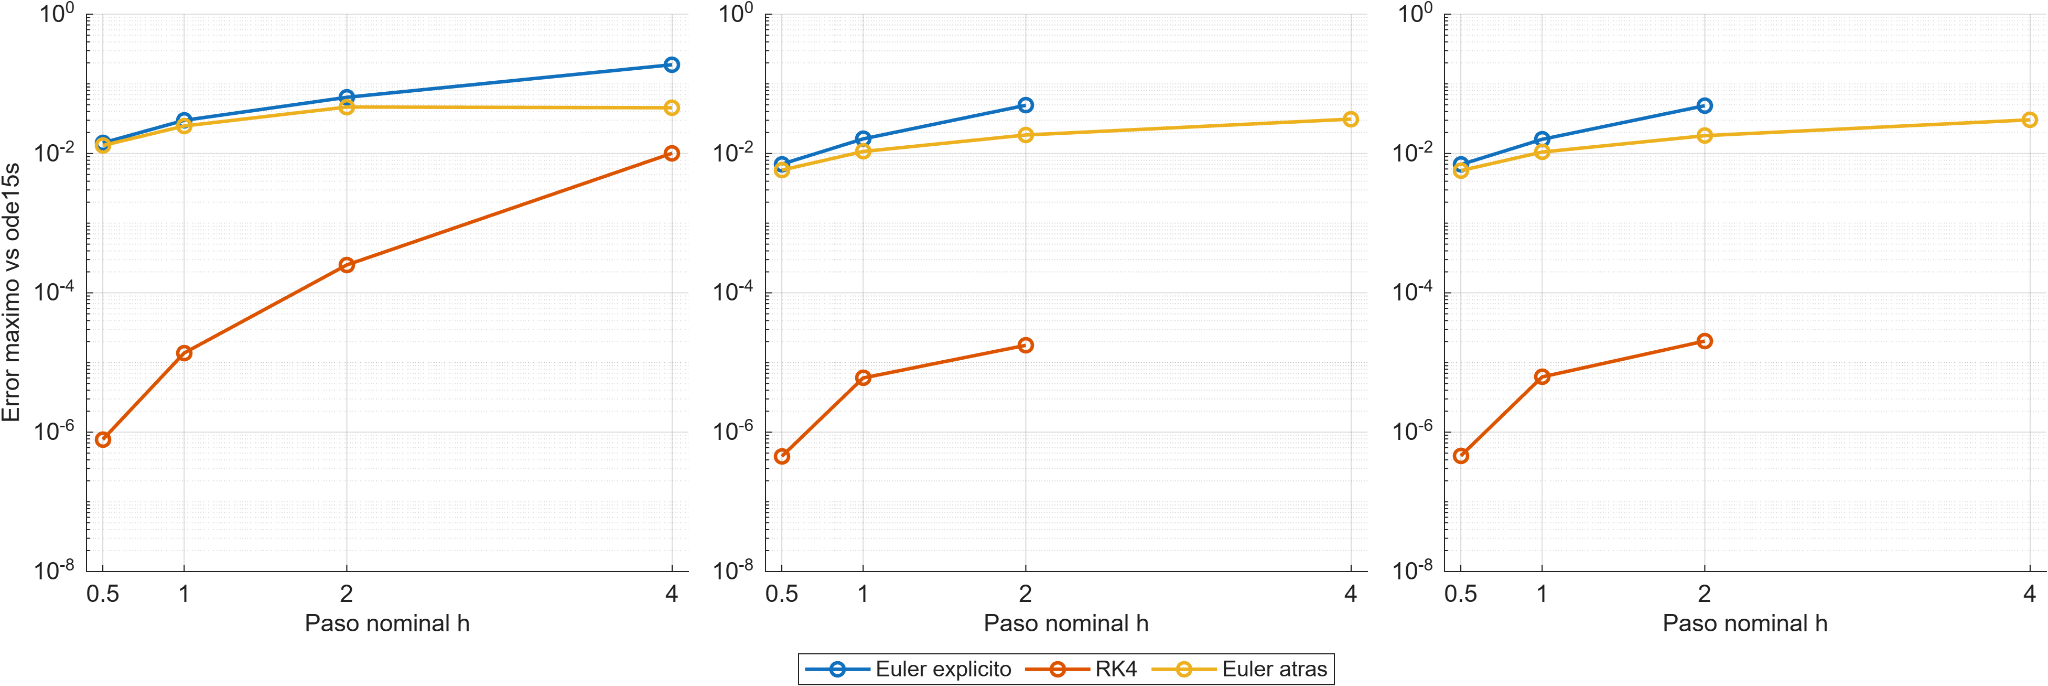
\includegraphics[width=0.91\textwidth]{imagenes/fig02_rigidez_estabilidad.png}
\caption{Error máximo frente a \texttt{ode15s} según el paso nominal para $\varepsilon=0.1$, $0.01$ y $0.001$ (paneles de izquierda a derecha). El eje vertical es logarítmico para distinguir los errores de RK4. Solo aparecen los casos admisibles.}
\label{fig:rigidez}
\end{figure*}

\subsection{Variación de parámetros}
Se varió un parámetro por ejecución, manteniendo fijos los restantes valores del conjunto exploratorio, con la condición inicial alternativa. La tabla~\ref{tab:parametricos} resume el intervalo de fracciones infectadas finales observado en el CSV exportado por el experimento 08. Todos los casos registrados finalizaron con estado \texttt{OK} y error máximo de conservación menor que $2.5\cdot10^{-15}$. Estos resultados cuantifican sensibilidad local al diseño experimental; no constituyen una calibración epidemiológica ni garantizan tendencias universales.
\begin{table}[!tbp]
\centering\footnotesize
\caption{Variación uniparamétrica: fracción infectada final en los extremos del barrido.}
\label{tab:parametricos}
\begin{tabular}{lcccc}
\toprule
Parámetro & Valor bajo & $I_f$ & Valor alto & $I_f$ \\
\midrule
$b_1$ & 0.5 & 0.3222 & 2.0 & 0.4429 \\
$b_2$ & 0.5 & 0.3892 & 2.0 & 0.2405 \\
$K$ & 0 & 0.3892 & 0.9 & 0.3222 \\
$\beta$ & 2 & 0.0206 & 8 & 0.3792 \\
\bottomrule
\end{tabular}
\par{\scriptsize\textit{Nota.} $I_f$: fracción infectada final; demás parámetros fijos.\par}
\end{table}

\begin{figure*}[!b]
\centering
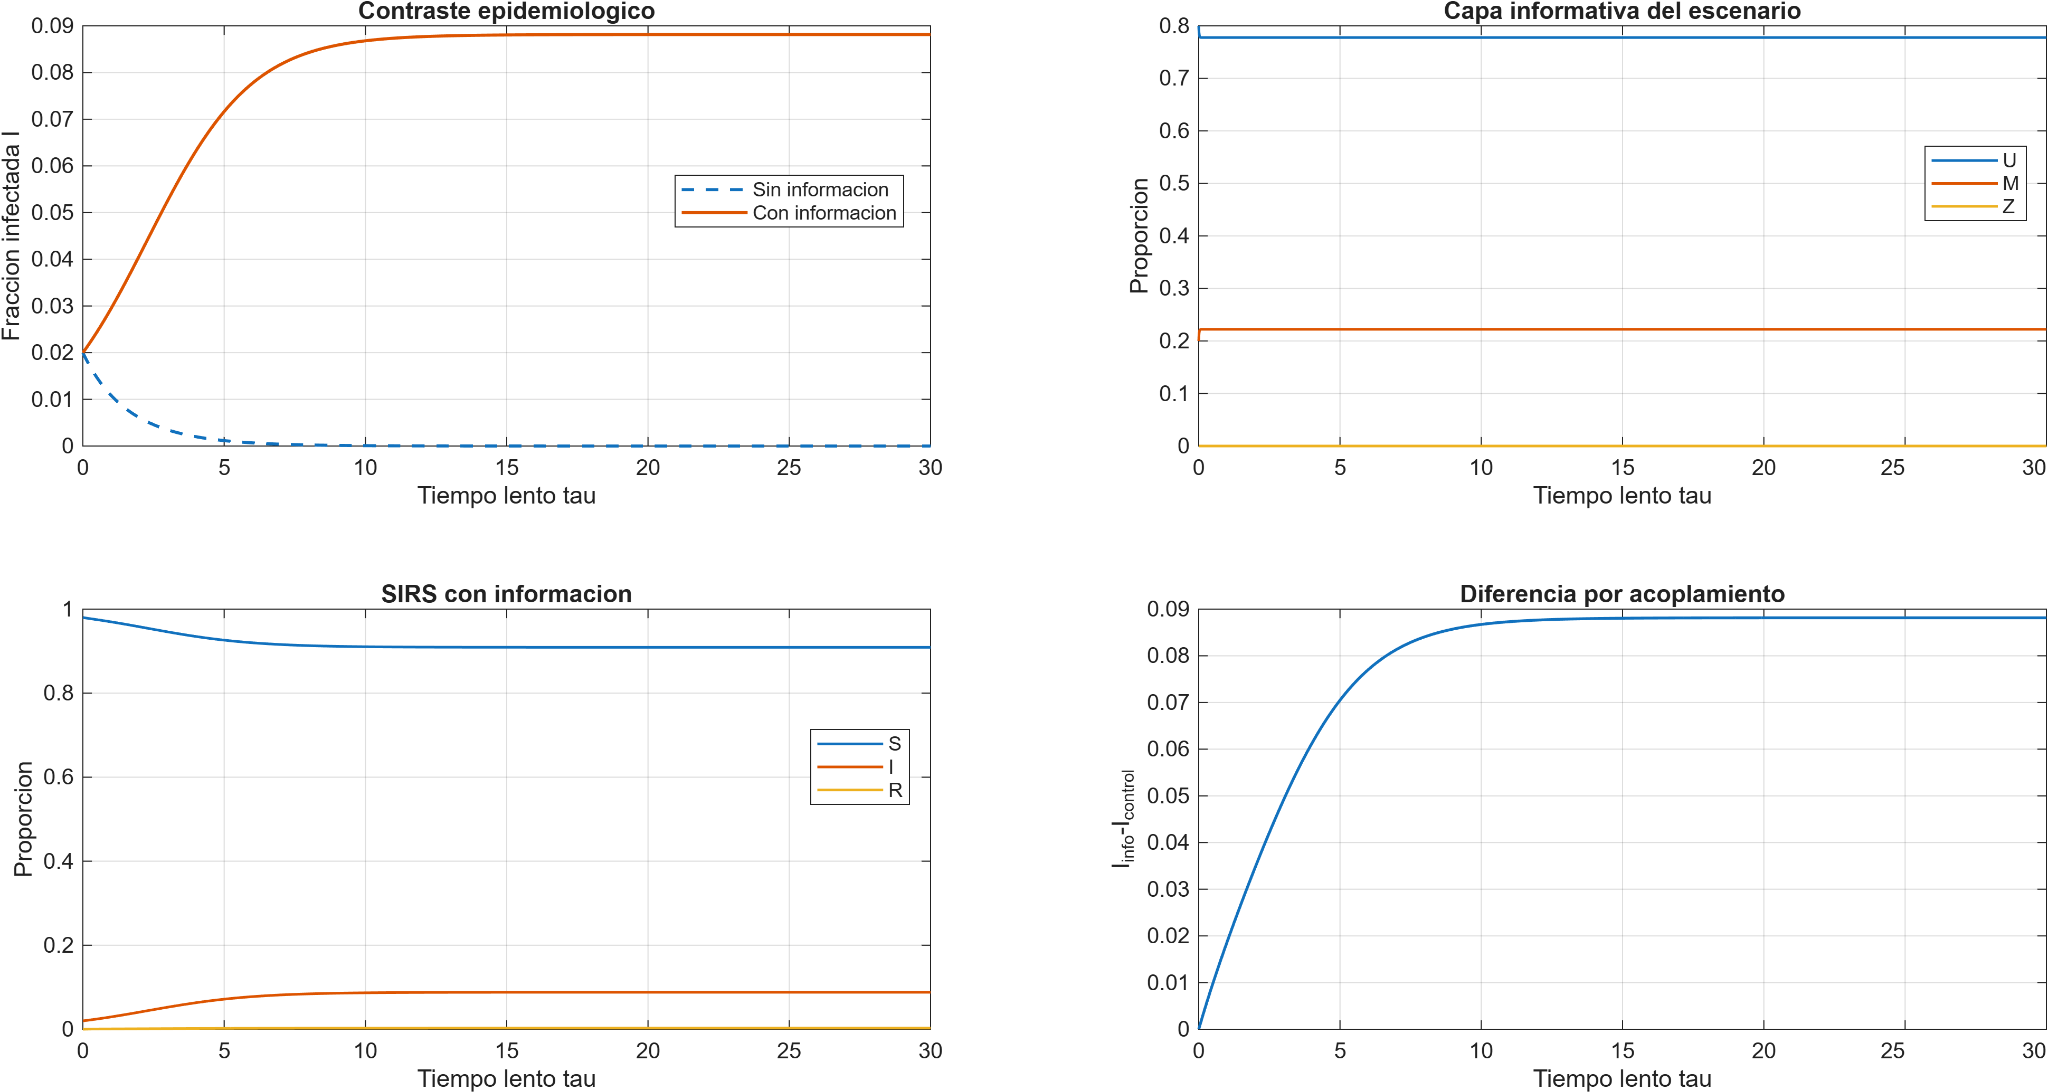
\includegraphics[width=0.72\textwidth]{imagenes/fig03_escenario_desinformacion.png}
\caption{Dinámica epidemiológica con desinformación y control sin difusión informativa. Programa MATLAB 07.}
\label{fig:desinformacion}
\end{figure*}

\subsection{Desinformación y escepticismo}
Se contrastó el efecto del acoplamiento social con un control informativo constante para dos conjuntos de parámetros. La tabla \ref{tab:epidemia} presenta las fracciones infectadas finales en tiempo lento $\tau=30$. En el escenario I, con desinformación, $I$ terminó alrededor de $0.08814$, frente a $1.65\cdot10^{-9}$ en el control. En el escenario II, con escepticismo, terminó en $1.51\cdot10^{-9}$, mientras el control finalizó aproximadamente en $0.08813$.

\begin{table}[t]
\centering\footnotesize
\caption{Fracción infectada al final de los escenarios epidemiológicos ($\tau=30$).}
\label{tab:epidemia}
\begin{tabular}{lrr}
\toprule Escenario & Control & Con acoplamiento \\ \midrule
I: desinformación & $1.6453\cdot10^{-9}$ & $0.08814414$ \\
II: escepticismo & $0.08812925$ & $1.5130\cdot10^{-9}$ \\
\bottomrule
\end{tabular}
\par{\scriptsize\textit{Nota.} Control: sin información; acoplamiento: con información.\par}
\end{table}

En las dos trayectorias acopladas, el error máximo de RK4 respecto a \texttt{ode15s} fue $2.82\cdot10^{-8}$ y $5.47\cdot10^{-8}$, respectivamente. Los errores de conservación estuvieron alrededor de $10^{-15}$ y las componentes permanecieron no negativas. Los controles y las curvas informativas se ilustran en las figuras \ref{fig:desinformacion} y \ref{fig:escepticismo}; representan únicamente los horizontes e hipótesis considerados.



En conjunto, el contraste de integradores mostró diferencias importantes en precisión y en admisibilidad a pasos grandes; al disminuir $\varepsilon$ creció el indicador espectral inicial y se requirió mayor atención a la estabilidad. Los dos escenarios de acoplamiento produjeron respuestas epidémicas opuestas dentro del horizonte simulado, sin que ello constituya una demostración de su comportamiento asintótico. El barrido de parámetros mostró diferencias apreciables en la infección final, sin violar la conservación poblacional en los casos registrados.

\begin{figure*}[!t]
\centering
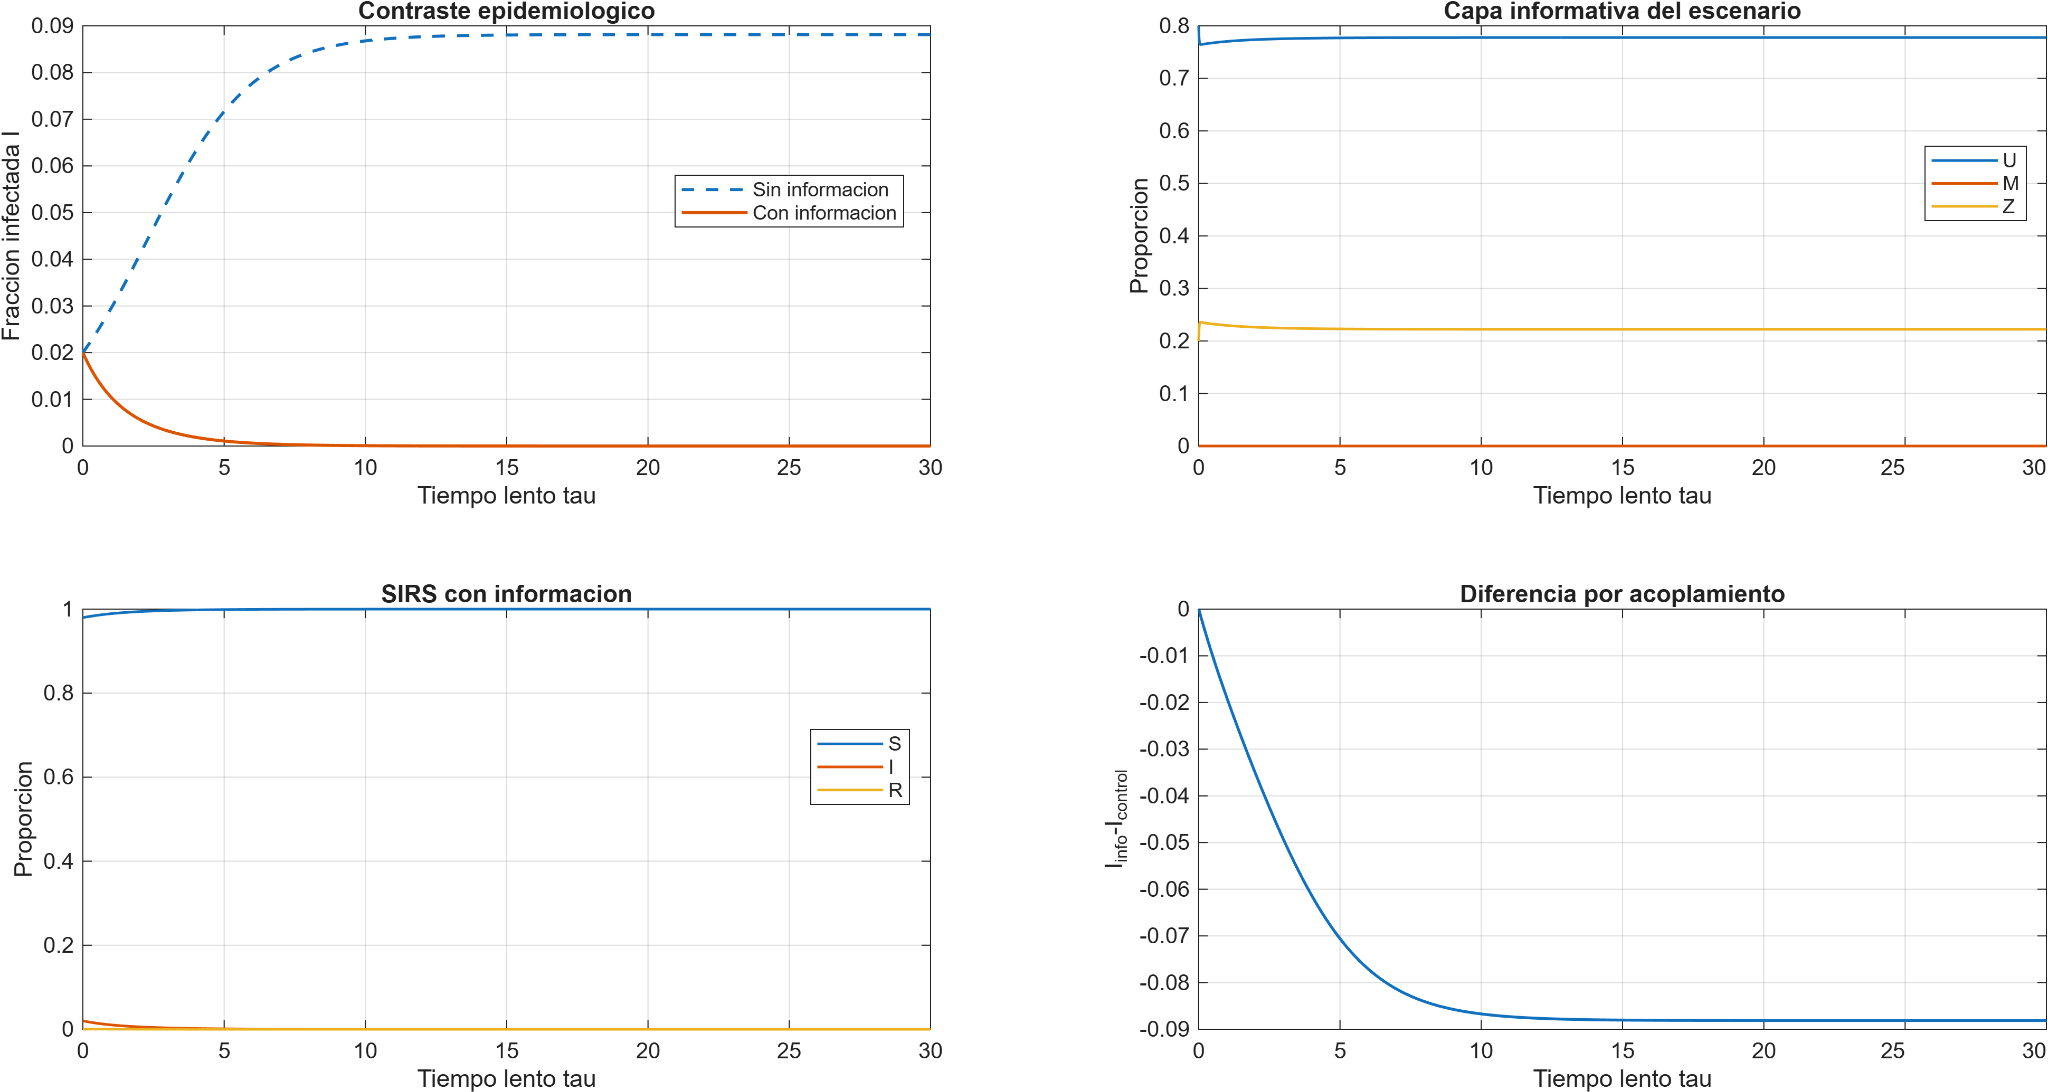
\includegraphics[width=0.72\textwidth]{imagenes/fig04_escenario_escepticismo.png}
\caption{Dinámica epidemiológica con escepticismo y control sin difusión informativa. Programa MATLAB 07.}
\label{fig:escepticismo}
\end{figure*}

\section{Discusión preliminar}
La comparación de integradores permitió separar dos conceptos que no deben confundirse: precisión y estabilidad. Con pasos moderados, RK4 alcanzó un error muy inferior al de ambos métodos de Euler, como se aprecia en la tabla \ref{tab:errores} y la figura \ref{fig:convergencia}. El descenso experimental de error de RK4 fue consistente con orden cuatro, mientras los métodos de Euler se comportaron aproximadamente como esquemas de primer orden. No obstante, el rendimiento observado depende del tamaño de paso, de la trayectoria y de la referencia numérica seleccionada. Asimismo, el número de evaluaciones de $\mathbf f$ no representa todo el costo computacional de Euler hacia atrás, que incluye construcción de jacobianas, Newton y Gauss--Seidel.

RKF45 fue especialmente competitivo en evaluaciones para los escenarios de precisión inicial, pero su paso fue adaptativo y sus condiciones no equivalieron a un paso fijo idéntico al de RK4. La corrección de la comparación en los nodos aceptados eliminó una discrepancia artificial de conservación que aparecía cuando se interpolaban externamente las trayectorias. Esa revisión puso de relieve la necesidad de validar no solo el integrador, sino también la forma de medir sus errores. Un estudio posterior debería variar las tolerancias de RKF45 y comparar costo frente a una misma meta de error.

El incremento de la razón espectral local con $1/\varepsilon$ fue compatible con la estructura rápido--lento de Bulai et al. (2024). Los fallos de admisibilidad de los métodos explícitos para pasos grandes, recogidos en la tabla \ref{tab:rigidez} y la figura \ref{fig:rigidez}, mostraron que un paso razonable para la dinámica epidemiológica puede resultar excesivo para la informativa. Sin embargo, el éxito de Euler hacia atrás no se interpretó como estabilidad incondicional del algoritmo completo: Gauss--Seidel puede no converger para ciertas matrices internas y se recurrió a rechazar pasos, verificando positividad y residuos. Estos mecanismos aumentaron las iteraciones y, en algunos casos, el número de pasos efectivo superó ampliamente el esperado con el paso nominal.

Finalmente, el contraste de los escenarios epidemiológicos de la tabla \ref{tab:epidemia} y las figuras \ref{fig:desinformacion}--\ref{fig:escepticismo} mostró variaciones marcadas en la infección asociadas con la presencia de una rama informativa particular. El primer escenario mantuvo una prevalencia apreciable en el horizonte simulado, mientras el control decayó; el segundo produjo el resultado opuesto. Los resultados son compatibles con el acoplamiento propuesto por Bulai et al. (2024), pero dependen de las condiciones iniciales y los parámetros elegidos. El estudio no constituye una estimación epidemiológica real ni una demostración de extinción asintótica. Quedan como limitaciones la ausencia de datos observados para calibración, el carácter local del indicador espectral, el rango finito de pasos explorados y la necesidad de contrastar formalmente la convergencia de las referencias antes de cerrar el paper final.

El barrido uniparamétrico complementó la comparación entre métodos: los valores finales de infección registrados dependieron de $b_1$, $b_2$, $K$ y $\beta$. La Tabla~\ref{tab:parametricos} presenta los extremos explorados; estas variaciones aisladas no permiten extrapolar conclusiones a todos los regímenes ni probar rebrotes no observados.

\clearpage
\section*{Anexos y código}
Los archivos de implementación en MATLAB (\texttt{.m} y \texttt{.mlx}), las figuras y las tablas de resultados se encuentran organizados en el repositorio del proyecto: \url{https://github.com/jmtimana/CC2104-UMZ-SIRS-Grupo8}. La reproducibilidad de los experimentos puede verificarse a partir de los scripts y los parámetros descritos en la Metodología.
\section*{Referencias}
 
\begin{flushleft}
\setlength{\parindent}{0pt}
\hangindent=1.27cm
\hangafter=1
Bulai, I. M., Sensi, M., \& Sottile, S. (2024). A geometric analysis of the SIRS compartmental model with fast information and misinformation spreading. \textit{Chaos, Solitons \& Fractals, 185}, Article 115104. \url{https://doi.org/10.1016/j.chaos.2024.115104}
 
\hangindent=1.27cm
\hangafter=1
Dahlquist, G. G. (1963). A special stability problem for linear multistep methods. \textit{BIT Numerical Mathematics, 3}(1), 27--43. \url{https://doi.org/10.1007/BF01963532}
 
\hangindent=1.27cm
\hangafter=1
da Silva, M. I., De Cezaro, A., Marques, J. C., Ferreira Nicola Gomes, A. C., \& Otazu Conza, A. (2023). The stiffness phenomena for the epidemiological SIR model: A numerical approach. \textit{Latin-American Journal of Computing, 10}(2). \url{https://doi.org/10.5281/zenodo.8067335}
 
\hangindent=1.27cm
\hangafter=1
Dembo, R. S., Eisenstat, S. C., \& Steihaug, T. (1982). Inexact Newton methods. \textit{SIAM Journal on Numerical Analysis, 19}(2), 400--408. \url{https://doi.org/10.1137/0719025}
 
\hangindent=1.27cm
\hangafter=1
Giambiagi Ferrari, C., Pinasco, J. P., \& Saintier, N. (2021). Coupling epidemiological models with social dynamics. \textit{Bulletin of Mathematical Biology, 83}(7), Article 74. \url{https://doi.org/10.1007/s11538-021-00910-7}
 
\hangindent=1.27cm
\hangafter=1
Hernández Guillén, J. D., \& Martín del Rey, A. (2018). Modeling malware propagation using a carrier compartment. \textit{Communications in Nonlinear Science and Numerical Simulation, 56}, 217--226. \url{https://doi.org/10.1016/j.cnsns.2017.08.011}
 
\hangindent=1.27cm
\hangafter=1
Jia, P., Wang, C., Zhang, G., \& Ma, J. (2019). A rumor spreading model based on two propagation channels in social networks. \textit{Physica A: Statistical Mechanics and its Applications, 524}, 342--353. \url{https://doi.org/10.1016/j.physa.2019.04.163}
 
\hangindent=1.27cm
\hangafter=1
Li, D., Xie, W., \& Han, D. (2024). Multi-information and epidemic coupling propagation considering indirect contact on two-layer networks. \textit{Applied Mathematics and Computation, 474}, Article 128700. \url{https://doi.org/10.1016/j.amc.2024.128700}
 
\hangindent=1.27cm
\hangafter=1
Paul, S., Mondal, S. P., \& Bhattacharya, P. (2016). Numerical solution of Lotka--Volterra prey-predator model by using Runge--Kutta--Fehlberg method and Laplace Adomain decomposition method. \textit{Alexandria Engineering Journal, 55}(1), 613--617. \url{https://doi.org/10.1016/j.aej.2016.01.033}
 
\hangindent=1.27cm
\hangafter=1
Rehman, A. U., Singh, R., \& Singh, J. (2022). Mathematical analysis of multi-compartmental malaria transmission model with reinfection. \textit{Chaos, Solitons \& Fractals, 163}, Article 112527. \url{https://doi.org/10.1016/j.chaos.2022.112527}
 
\hangindent=1.27cm
\hangafter=1
Shampine, L. F., \& Gear, C. W. (1979). A user's view of solving stiff ordinary differential equations. \textit{SIAM Review, 21}(1), 1--17. \url{https://doi.org/10.1137/1021001}
 
\hangindent=1.27cm
\hangafter=1
Städter, P., Schälte, Y., Schmiester, L., Hasenauer, J., \& Stapor, P. L. (2021). Benchmarking of numerical integration methods for ODE models of biological systems. \textit{Scientific Reports, 11}(1), Article 2696. \url{https://doi.org/10.1038/s41598-021-82196-2}
\end{flushleft}

\end{document}
